\subsection{Multi-Dimensional Evaluation Harness}
\label{sec:method_evalharness}

\subsubsection{Judge Configuration via YAML}

The evaluation harness is configured independently from the runtime under test. A separate YAML file specifies the judge model, decoding parameters, and prompt templates for each scoring function. This separation is intentional. It allows a stronger or more stable model to serve as the judge, and it lets researchers redefine the evaluation criteria without editing the evaluation code. In practice, we recommend using a deterministic judge configuration with temperature fixed at zero so that repeated runs remain comparable.

\begin{figure}[t]
\centering
\begin{minipage}{0.92\linewidth}
\begin{lstlisting}[basicstyle=\color{blue}\small\ttfamily]
name: "Default Judge Prompts"
model:
  provider: azure
  name: gpt-4o
  parameters: {temperature: 0.0}
prompts:
  assertion_check: |
    Verify whether the response satisfies each assertion.
  citation_relevance: |
    Judge the relevance of tool results to the query.
  response_citation: |
    Judge whether cited IDs are real, relevant, and
    grounded in the tool trace.
\end{lstlisting}
\end{minipage}
\caption{Condensed judge configuration illustrating independent control of the evaluation model and prompt templates.}
\label{lst:judge_yaml}
\end{figure}

\subsubsection{Configurable Evaluation Metrics}

EABench separates the \emph{harness logic} from the \emph{evaluation criteria}. Researchers specify what to measure entirely through configuration; no code changes are required to add, replace, or retune a metric.

\textbf{Judge-based metrics} are defined by prompt templates in the judge YAML file (Figure~\ref{lst:judge_yaml}). Each template receives the agent's query, response, and tool trace, and returns a score in $[0,1]$ with an explanation. Any number of judge prompts can be registered; common patterns include:
\begin{itemize}[leftmargin=*,itemsep=2pt,topsep=4pt]
  \item \textbf{Factual assertion checking.} A prompt that verifies whether each gold-standard assertion in the evaluation case is satisfied by the agent's response. The per-case score is a pass fraction over all assertions.
  \item \textbf{Retrieval quality.} A prompt that jointly evaluates tool selection, evidence relevance, and response grounding---checking whether the agent's answer faithfully reflects what was retrieved rather than hallucinating.
  \item \textbf{Citation grounding.} A prompt that inspects the response's references section: whether it exists, whether cited artifact IDs appear in the tool trace, and whether inline citation markers are present.
  \item \textbf{Derived aggregates.} Scores derived from two or more judge outputs---e.g., the mean of retrieval quality and citation grounding---to summarize end-to-end evidence handling.
\end{itemize}

\textbf{Deterministic diagnostics} are extracted from the tool trace and response text without an LLM call. They are always computed regardless of judge configuration and serve as interpretable proxies for agent behavior:
\begin{itemize}[leftmargin=*,itemsep=2pt,topsep=4pt]
  \item \textbf{Retrieved-item count.} Total evidence items returned across all search tool calls.
  \item \textbf{Response citation count.} Number of structured reference entries emitted in the final answer.
  \item \textbf{Token usage, tool-call count.} Operational cost and trajectory efficiency.
\end{itemize}

\textbf{Pass/fail threshold.} Whether a case is marked as passed is controlled by threshold parameters applied to any subset of the judge scores. Setting tighter thresholds raises the bar for correctness and grounding; researchers can calibrate these to match the compliance requirements of their target deployment context.

\begin{table}[h]
\centering
\caption{Metrics reported by the EABench evaluation harness.}
\label{tab:eval_metrics}
\small
\begin{tabular}{p{0.22\linewidth}p{0.16\linewidth}p{0.52\linewidth}}
\toprule
\textbf{Metric} & \textbf{Type} & \textbf{Interpretation} \\
\midrule
Assertion score & Judge-based & Fraction of natural-language assertions satisfied by the final answer \\
Tool search result relevance & Judge-based & Whether the selected tools and retrieved evidence were appropriate and faithfully reflected in the answer \\
Response citation score & Judge-based & Whether the final answer cites real, relevant artifacts and includes grounded references \\
Combined citation score & Derived & Mean of tool relevance and response citation scores \\
Tool search result number & Deterministic & Number of retrieved evidence items surfaced across search tool calls \\
Response citation number & Deterministic & Number of references emitted by the agent in the final answer \\
Token usage, tool-call count & Deterministic & Operational cost and efficiency of the agent trajectory \\
\bottomrule
\end{tabular}

\end{table}

\begin{figure}[t]
\centering
%\fbox{\parbox{0.96\linewidth}{%
%\vspace{4pt}
%\small\color{blue}\itshape\raggedright
%\textbf{[Figure placeholder --- generation pending.]}
%A vertical funnel-and-merge scoring pipeline diagram.
%\textbf{Top input block (deep blue, full width):} A wide rectangle labeled ``Agent Response + Tool Trace + Source Citations'' with embedded icons: a document icon (response), a chain-link icon (tool trace), and a citation-list icon (source citations).
%Below the input block, a downward arrow fans into \textbf{three parallel vertical scoring tracks} separated by column dividers:
%\textbf{Track~1 (left, amber) --- Citation Relevance Score:}
%A ``Judge LLM'' rounded box with two annotation badges: ``prompt-configurable'' and ``threshold-configurable.''
%Inside the box, a small visual: retrieved tool results $\rightarrow$ relevance check against query and access list $\rightarrow$ score bar.
%Output: a horizontal score bar labeled ``0.0 \ldots 1.0'' in amber tone.
%\textbf{Track~2 (center, orange) --- Assertion Check Score:}
%A ``Judge LLM'' rounded box. Inside: assertions listed individually, each checked True/False against the response.
%Output: a pass-fraction score bar labeled ``0.0 \ldots 1.0'' in orange tone.
%Below the two parallel tracks (TS-Rel and RC-Rel), a merge node computes the equal-weight mean (combined citation score).
%The combined score and the assertion score feed a final Pass/Fail decision node.
%To the far right, outside the main pipeline, a vertically stacked \textbf{Deterministic Diagnostics} column (light gray): Latency, Token Usage, Tool-call Count, Evidence Items---each as a labeled metric box.
%Color scheme: input block in deep blue; Track~1 amber; Track~2 orange; Track~3 teal; merge zone and final gauge in green; deterministic column gray.
%\vspace{4pt}
%}}
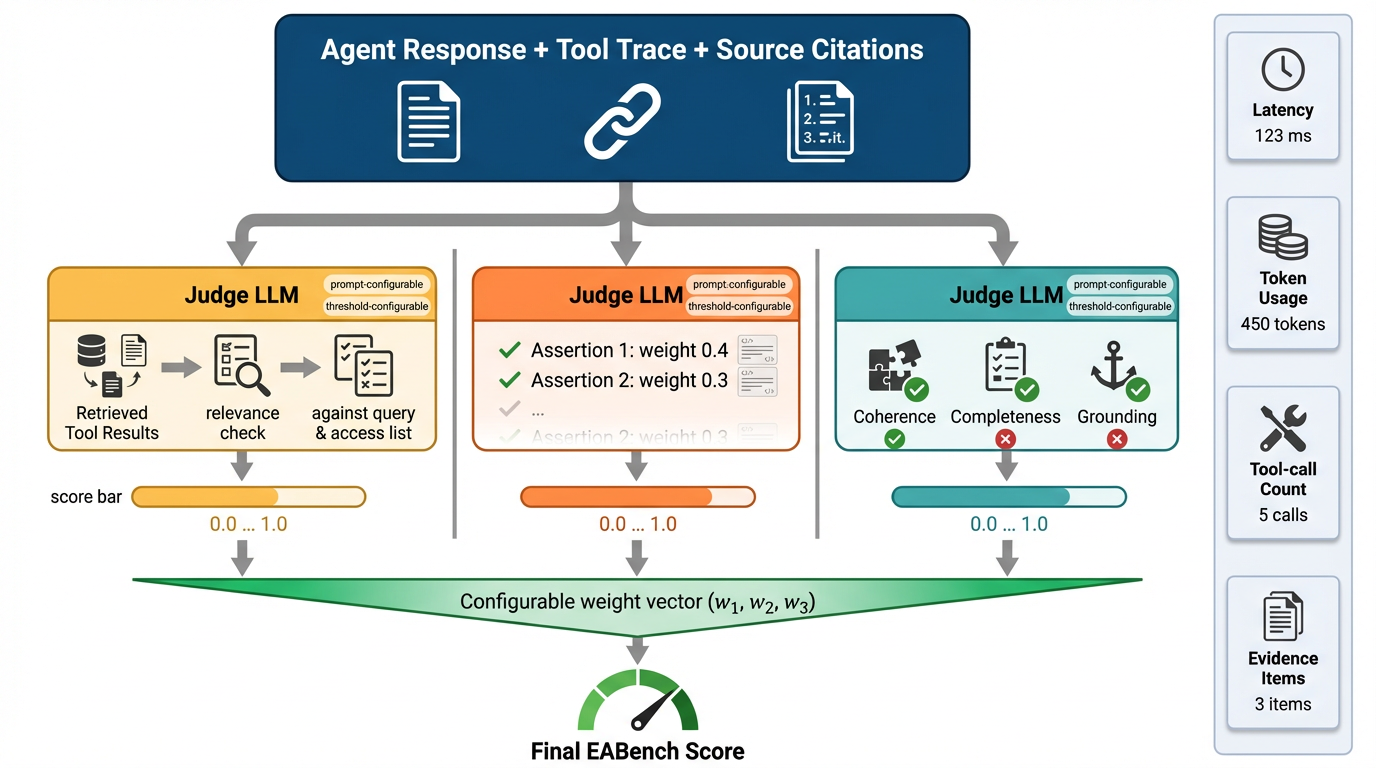
\includegraphics[width=0.9\textwidth]{figures/LLM-as-a-judge-eabench.png}
\caption{EABench multi-dimensional evaluation harness. Two independently configurable LLM-judge tracks score tool-search relevance and response-citation quality; their equal-weight average forms the combined citation score. The assertion score is computed by a third judge call. All three judge scores are reported alongside deterministic diagnostics for operational profiling.}
\label{fig:eval_harness}
\end{figure}

\subsubsection{Pass/Fail Criteria}

A case is marked as passed when both of the following conditions hold simultaneously:
\begin{itemize}[leftmargin=*,itemsep=2pt,topsep=4pt]
  \item \textbf{Assertion score $\geq 0.75$.} At least 75\% of the natural-language assertions are satisfied. This threshold reflects enterprise contexts in which a response missing more than one in four factual requirements is operationally unacceptable.
  \item \textbf{Response-citation quality $\geq 0.7$.} The final answer must include a sufficiently grounded references section. This gate ensures that a plausible-sounding response is still marked as failed if it cites hallucinated artifacts.
\end{itemize}
This dual criterion encodes an important design principle: correctness and grounding are jointly necessary for enterprise-agent success. An agent that satisfies all assertions but fabricates its citations fails the grounding gate; an agent with a well-formed references section that misses key facts fails the correctness gate.

\textcolor{blue}{We do not currently report a human-annotator validation study of assertion grounding, satisfiability, and inter-rater agreement; the assertion-generation pipeline is instead validated indirectly through judge--judge agreement checks and through a post-hoc keyword-based audit of query-type coverage (Section~\ref{sec:experiments}). We treat a full human-annotation study as an open validation task (Section~\ref{sec:threats}).}

\subsubsection{Side-by-Side Comparison and Diagnostics}

For comparative studies, EABench can evaluate two agent configurations on the same case and ask a judge model to declare a winner. These pairwise judgments support win-rate analyses and Bradley--Terry modeling, while the underlying per-case metric vectors support paired tests such as the Wilcoxon signed-rank test. Because the result structure stores the full response, tool trace, assertion outcomes, and citation logs, comparative findings are accompanied by diagnostics that explain why one agent won rather than only whether it won.

\subsubsection{User-Level Experience Simulation}

Evaluation is always grounded in a requesting user context. Before each case is run, the search engine is bound to \texttt{case.user\_id}, and access-control rules are enforced consistently across search results, citation verification, and debugging views. This design allows the same tenant to support engineer, manager, and contractor personas without maintaining separate corpora, and it turns access control into a benchmarked capability rather than an external precondition.